\documentclass{article}
\usepackage{neurips_2024}

% Core packages
\usepackage{amsmath,amssymb,amsthm}
\usepackage{graphicx}
\usepackage{tikz}
\usetikzlibrary{arrows.meta,positioning,calc,backgrounds}
\usepackage{booktabs}
\usepackage{multirow}
\usepackage{algorithm}
\usepackage{algorithmic}
\usepackage{microtype}
\usepackage{xcolor}
\usepackage{hyperref}
\usepackage{url}
\hypersetup{colorlinks=true,linkcolor=black,citecolor=black,urlcolor=black}

% Colours
\definecolor{maskblue}{RGB}{55,110,170}
\definecolor{ctxgray}{RGB}{215,215,215}
\definecolor{phgray}{RGB}{130,130,130}

% Paper commands
\newcommand{\aomt}{\textsc{AOMT}}
\newcommand{\Lcal}{\mathcal{L}}
\newcommand{\Ucal}{\mathcal{U}}
\newcommand{\Dcal}{\mathcal{D}}
\newcommand{\Ccal}{\mathcal{C}}
\newcommand{\Tcal}{\mathcal{T}}
\newcommand{\NLL}{\mathrm{NLL}}

% Placeholder helpers
\newcommand{\PLACEHOLDER}[1]{\textcolor{phgray}{\textit{[#1]}}}
\newcommand{\figplaceholder}[2][5.5cm]{%
  \begin{center}
    \fcolorbox{black!30}{black!5}{%
      \parbox[c][#1]{\linewidth-2\fboxsep-2\fboxrule}{%
        \centering\color{phgray}\small\textit{#2}%
      }%
    }%
  \end{center}%
}

% Theorem environments
\newtheorem{proposition}{Proposition}
\newtheorem{definition}{Definition}
\newtheorem{remark}{Remark}

\title{Any-Order Masked Training for Trajectory-Level\\
       Supervised Learning in LLM-Based Agents}

\author{Anonymous authors\\Paper under double-blind review}

\begin{document}

\maketitle

\begin{abstract}
Supervised fine-tuning (SFT) on expert trajectories is the dominant paradigm for
bootstrapping LLM-based agents, yet it commits to a single, rigid \emph{training
order}: the full causal prefix is context, the next action is the only target.
A trajectory of length $T$ contains $O(2^T)$ possible context/target assignments;
standard SFT exploits exactly $T$ of them.
We propose \textbf{Any-Order Masked Training (\aomt{})}, a reward-free offline
paradigm that treats agent learning as a trajectory-level reconstruction problem.
At each training step, an arbitrary subset of observation and action
\emph{units}---whole semantic spans, not individual tokens---is randomly masked;
the remaining units serve as bidirectional context; and a masked diffusion language
model reconstructs the masked units in a single forward pass.
Resampling the mask across epochs, the same expert trajectory simultaneously
supervises a large family of conditional distributions.
We prove that standard SFT and the offline variant of ALEE's Implicit World
Modeling objective \citep{zhang2025alee} are degenerate special cases of \aomt{}
under constrained mask samplers.
We evaluate on ALFWorld, ScienceWorld, and WebShop, and introduce
\emph{observation-masked NLL} as a novel metric for implicit world-model quality.
\PLACEHOLDER{Final results and main findings to be inserted after experiments complete.}
\end{abstract}

\section{Introduction}
\label{sec:intro}

Supervised fine-tuning (SFT) on expert demonstrations is the dominant starting
point for LLM-based agents \citep{deng2023mind2web,zeng2023agenttuning,yao2023react}.
The standard objective---autoregressive next-action prediction---has a precise
structural limitation: it commits to a \emph{single, fixed} assignment of trajectory
elements to the roles of context and target.

\begin{definition}[Training Order]
\label{def:order}
A \emph{training order} $\sigma$ is a function
$\sigma\colon \Ucal(\tau) \to \{\texttt{context},\, \texttt{target}\}$
partitioning the units of a trajectory $\tau$ into a context set $\Ccal_\sigma$
and a target set $\Tcal_\sigma$ for a single training update.
\end{definition}

Standard SFT always uses the same order: every preceding observation and action
is context; the next action is the only target. A trajectory of length $T$ contains
$O(2^T)$ possible context/target assignments, of which standard SFT exploits
exactly $T$---one per action step. Recent alternatives such as
ALEE \citep{zhang2025alee} introduce richer signals but each fix a single training
order and require either live environment interaction or human annotation.

\paragraph{This paper.}
We propose \textbf{Any-Order Masked Training (\aomt{})}, which removes the
single-order constraint entirely. At each training step, an arbitrary subset of
whole observation and action \emph{units} is randomly masked; the remaining units
serve as bidirectional context; and a masked diffusion language model
\citep{nie2025llada} reconstructs all masked units in a single forward pass.
Over multiple epochs, the same trajectory appears under many distinct
context/target assignments---inducing any-order learning without additional data
collection, environment interaction, or reward signals.

We use LLaDA~2.0 \citep{bie2025llada20} as our base model: masked diffusion LMs
natively support full bidirectional attention and are structurally designed for
span reconstruction. Masking is applied at the \emph{unit level} (whole
observations or actions) rather than at the token level, preventing partial-token
information leakage and forcing reconstruction to rely on inter-unit trajectory
structure.

\paragraph{Contributions.}
\textbf{(1)} \textbf{\aomt{}}: a reward-free offline training objective applying
unit-level random masking to agent trajectories, extracting richer supervision from
a fixed expert corpus.
\textbf{(2)} \textbf{Formal unification} (Proposition~\ref{prop:subsumption}):
standard SFT and offline ALEE-IWM are degenerate special cases of \aomt{}.
\textbf{(3)} \textbf{Observation-masked NLL}: a novel metric for implicit
world-model quality, naturally supported by masked DLMs.
\textbf{(4)} \textbf{Empirical evaluation} on ALFWorld, ScienceWorld, and WebShop
with ablations and robustness analysis.

\begin{figure}[t]
  \centering
  % figures/method_overview.tex  — \input inside figure environment
% Uses \resizebox{\textwidth}{!}{...} to guarantee fit on 5.5in ICLR page.
\resizebox{\textwidth}{!}{%
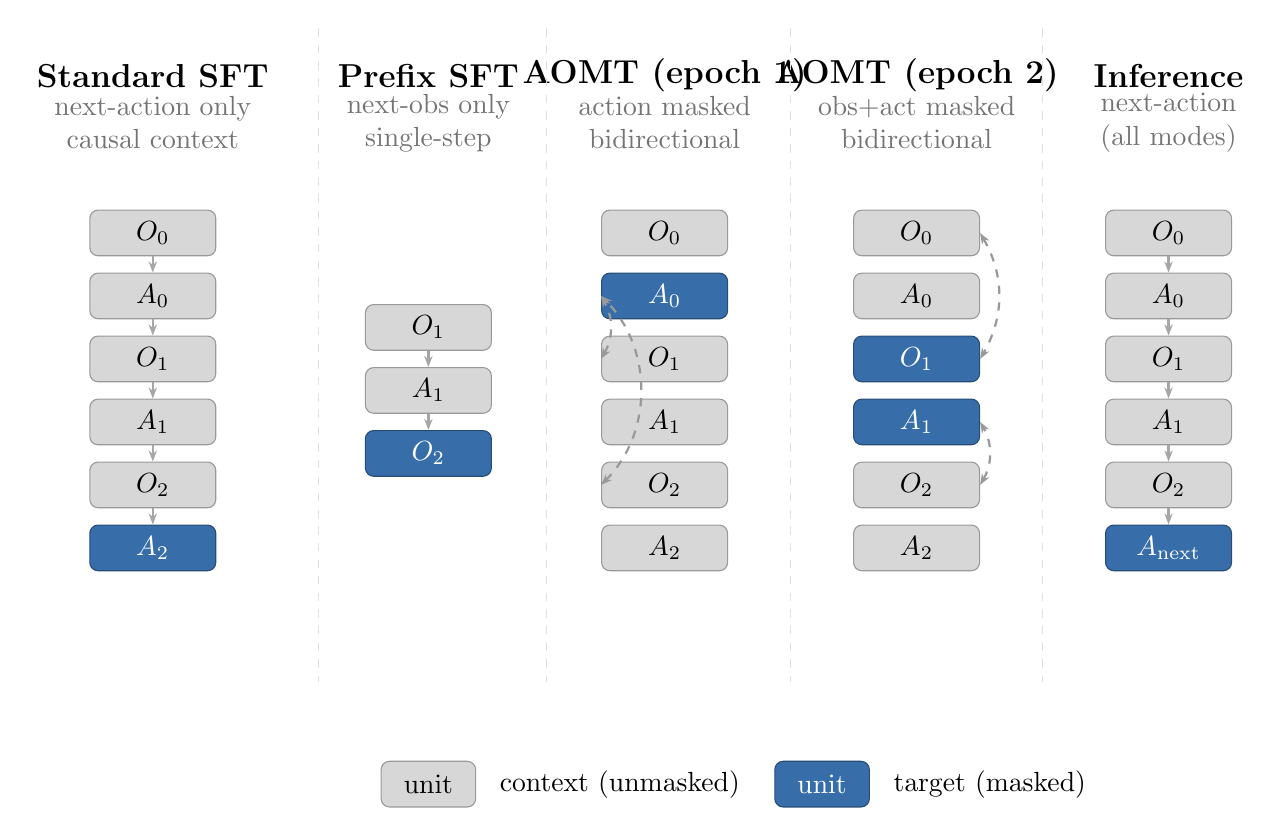
\begin{tikzpicture}[
  font=\normalsize,
  box/.style={draw, rounded corners=3pt,
              minimum width=1.6cm, minimum height=0.58cm,
              text centered, inner sep=3pt},
  ctx/.style={box, fill=ctxgray, draw=black!40},
  tgt/.style={box, fill=maskblue, draw=maskblue!70!black, text=white},
  hd/.style={font=\large\bfseries, align=center},
  sub/.style={font=\normalsize, align=center, text=black!55},
  arr/.style={-{Stealth[length=4pt]}, thick, black!35},
  biarr/.style={{Stealth[length=4pt]}-{Stealth[length=4pt]}, thick, dashed, black!40},
]

% Column x-centres (spacing chosen so total width ≈ 300pt before resizebox)
\def\ca{0}
\def\cb{3.5}
\def\cc{6.5}
\def\cd{9.7}
\def\ce{12.9}
\def\rs{0.8}   % row step (y)

%% ---- COLUMN HEADERS ----
\node[hd]  at (\ca, 2.0)  {Standard SFT};
\node[sub] at (\ca, 1.4)  {next-action only\\causal context};

\node[hd]  at (\cb, 2.0)  {Prefix SFT};
\node[sub] at (\cb, 1.4)  {next-obs only\\single-step};

\node[hd]  at (\cc, 2.0)  {\aomt{} (epoch 1)};
\node[sub] at (\cc, 1.4)  {action masked\\bidirectional};

\node[hd]  at (\cd, 2.0)  {\aomt{} (epoch 2)};
\node[sub] at (\cd, 1.4)  {obs+act masked\\bidirectional};

\node[hd]  at (\ce, 2.0)  {Inference};
\node[sub] at (\ce, 1.4)  {next-action\\(all modes)};

%% ---- COLUMN 1: Standard SFT (causal) ----
\node[ctx] (s0) at (\ca,  0)        {$O_0$};
\node[ctx] (s1) at (\ca, -\rs)      {$A_0$};
\node[ctx] (s2) at (\ca, -2*\rs)    {$O_1$};
\node[ctx] (s3) at (\ca, -3*\rs)    {$A_1$};
\node[ctx] (s4) at (\ca, -4*\rs)    {$O_2$};
\node[tgt] (s5) at (\ca, -5*\rs)    {$A_2$};
\foreach \a/\b in {s0/s1,s1/s2,s2/s3,s3/s4,s4/s5}{\draw[arr](\a)--(\b);}

%% ---- COLUMN 2: Prefix SFT ----
\node[ctx] (p0) at (\cb, -1.5*\rs)  {$O_1$};
\node[ctx] (p1) at (\cb, -2.5*\rs)  {$A_1$};
\node[tgt] (p2) at (\cb, -3.5*\rs)  {$O_2$};
\draw[arr](p0)--(p1); \draw[arr](p1)--(p2);

%% ---- COLUMN 3: AOMT epoch 1 (action masked) ----
\node[ctx] (e0) at (\cc,  0)        {$O_0$};
\node[tgt] (e1) at (\cc, -\rs)      {$A_0$};
\node[ctx] (e2) at (\cc, -2*\rs)    {$O_1$};
\node[ctx] (e3) at (\cc, -3*\rs)    {$A_1$};
\node[ctx] (e4) at (\cc, -4*\rs)    {$O_2$};
\node[ctx] (e5) at (\cc, -5*\rs)    {$A_2$};
% bidirectional context arrows: future units → masked A0
\draw[biarr] (e2.west) to[bend right=30] (e1.west);
\draw[biarr] (e4.west) to[bend right=45] (e1.west);

%% ---- COLUMN 4: AOMT epoch 2 (obs + act masked) ----
\node[ctx] (f0) at (\cd,  0)        {$O_0$};
\node[ctx] (f1) at (\cd, -\rs)      {$A_0$};
\node[tgt] (f2) at (\cd, -2*\rs)    {$O_1$};
\node[tgt] (f3) at (\cd, -3*\rs)    {$A_1$};
\node[ctx] (f4) at (\cd, -4*\rs)    {$O_2$};
\node[ctx] (f5) at (\cd, -5*\rs)    {$A_2$};
\draw[biarr] (f0.east) to[bend left=30] (f2.east);
\draw[biarr] (f4.east) to[bend right=30] (f3.east);

%% ---- COLUMN 5: Inference ----
\node[ctx] (i0) at (\ce,  0)        {$O_0$};
\node[ctx] (i1) at (\ce, -\rs)      {$A_0$};
\node[ctx] (i2) at (\ce, -2*\rs)    {$O_1$};
\node[ctx] (i3) at (\ce, -3*\rs)    {$A_1$};
\node[ctx] (i4) at (\ce, -4*\rs)    {$O_2$};
\node[tgt] (i5) at (\ce, -5*\rs)    {$A_\text{next}$};
\foreach \a/\b in {i0/i1,i1/i2,i2/i3,i3/i4,i4/i5}{\draw[arr](\a)--(\b);}

%% ---- Column dividers ----
\foreach \x in {2.1, 5.0, 8.1, 11.3}{
  \draw[black!12, dashed] (\x, 2.6) -- (\x, -5.7);
}

%% ---- Legend ----
\node[ctx, minimum width=1.2cm] (lc) at (3.5, -7.0) {unit};
\node[right=5pt of lc, font=\normalsize] {context (unmasked)};
\node[tgt, minimum width=1.2cm] (lt) at (8.5, -7.0) {unit};
\node[right=5pt of lt, font=\normalsize] {target (masked)};

\end{tikzpicture}%
}

  \caption{%
    \textbf{Any-Order Masked Training vs.\ prior single-order methods.}
    Standard SFT and Prefix SFT (offline IWM) each fix one training order.
    \aomt{} resamples an arbitrary unit-level mask each step, exposing the same
    trajectory under many context/target assignments across epochs.
    Inference is always next-action generation.
  }
  \label{fig:method_overview}
\end{figure}

\section{Related Work}
\label{sec:related}

\paragraph{SFT for LLM agents.}
Behavioural cloning on expert trajectories bootstraps LLM agents effectively
\citep{yao2022webshop,deng2023mind2web,zeng2023agenttuning,hong2024cogagent},
but generalises poorly out-of-distribution because the agent never reasons about
downstream consequences of its actions \citep{chu2025sft}.

\paragraph{Data-collection paradigms.}
ALEE \citep{zhang2025alee} trains on next-state prediction using self-generated
rollouts, requiring live environment access plus a separate SFT stage.
ETO \citep{song2024eto} collects failure trajectories for DPO-style contrastive
learning; IPR \citep{zhang2024ipr} adds step-level reward estimation.
All three require rollouts; ETO and IPR additionally require reward signals.
\aomt{} operates on the same offline corpus as standard SFT, innovating on the
\emph{objective axis} rather than the data axis---the two are orthogonal and
composable.

\paragraph{Masked diffusion LMs.}
LLaDA \citep{nie2025llada} learns bidirectional conditional distributions
via a variational bound on token-level NLL.
LLaDA~2.0 \citep{bie2025llada20} scales this to 16B/100B parameters (MoE),
with a SFT protocol that maps directly onto \aomt{}'s context/target distinction.
XLNet \citep{yang2019xlnet} pursues any-order learning via token-level permutation,
incurring two-stream attention overhead and a train--inference discrepancy;
\aomt{} operates at the coarser, semantically meaningful trajectory-unit level.

\paragraph{Masked objectives for agents.}
STeP \citep{chen2023step} and AGENTBANK/SAMOYED \citep{zeng2023agenttuning}
use token-level masking as a loss filter on a fixed causal objective.
Neither varies the context/target assignment nor employs bidirectional context.

\section{Method}
\label{sec:method}

\subsection{Setup and Notation}

A trajectory of length $T$ is the interleaved sequence
$\tau = (O_0, A_0, O_1, A_1, \ldots, O_{T-1}, A_{T-1}, O_T)$,
where $O_t \in \mathcal{O}$ and $A_t \in \mathcal{A}$ are multi-token text
spans called \emph{trajectory units}, with unit set
$\Ucal(\tau) = \{O_0, A_0, \ldots, O_T\}$, $|\Ucal| = 2T+1$.
An offline expert dataset $\Dcal = \{\tau^{(n)}\}_{n=1}^N$ is the sole training
source; \aomt{} uses no environment interaction or reward signal.

Standard SFT fixes $\sigma_\text{SFT}$: units $\{O_0,\ldots,O_t\}$ are context,
$A_t$ is the target, for each $t$, exploiting exactly $T$ of the $2^{2T+1}$
possible context/target partitions.

\begin{remark}
\label{rem:fraction}
Standard SFT exploits a fraction $T/2^{2T+1}$ of possible context/target
partitions---exponentially vanishing in $T$.
\end{remark}

\subsection{Any-Order Masked Training}
\label{sec:aomt_core}

A binary unit-level mask $m \in \{0,1\}^{|\Ucal|}$ partitions units into masked
targets $\Tcal(m) = \{u_i : m_i = 1\}$ and context $\Ccal(m) = \{u_i : m_i = 0\}$,
with $m_i \stackrel{\text{iid}}{\sim} \mathrm{Bernoulli}(p)$.
All tokens of masked units are replaced by \texttt{[MASK]}; context tokens are
unchanged. The \aomt{} objective is:
\begin{equation}
  \Lcal_{\text{AOMT}} =
    \mathbb{E}_{\tau \sim \Dcal}\;
    \mathbb{E}_{m \sim \mathrm{Mask}(p)}\;
    \left[
      -\sum_{u_i \in \Tcal(m)} \log p_\theta\!\left(u_i \mid \Ccal(m)\right)
    \right],
  \label{eq:aomt}
\end{equation}
where $p_\theta$ attends bidirectionally over all context units.
The mask is resampled at every training step; across epochs, the same trajectory
appears under many distinct assignments.

\paragraph{Why unit-level masking.}
Token-level masking on an action such as \texttt{``heat potato with oven''} can
leave partial cues visible, letting the model complete the action rather than
reason from trajectory context. Unit-level masking removes this shortcut and
aligns the loss with the semantic granularity at which agent decisions are made.

\paragraph{Training vs.\ inference.}
At inference, all \aomt{} models behave identically to standard SFT: the current
observation history is context and the next action is generated via LLaDA~2.0's
iterative unmasking \citep{bie2025llada20}. No observation prediction is
performed at test time.

\subsection{AOMT Subsumes Prior Single-Order Methods}

\begin{proposition}[Subsumption]
\label{prop:subsumption}
\emph{(i)} Standard SFT is the special case of \aomt{} with the mask sampler
constrained to always mask $A_t$ with causal context $\{O_0,\ldots,O_t\}$.
\emph{(ii)} Offline ALEE-IWM is the special case of \aomt{} with the mask
sampler constrained to always mask $O_{t+1}$ with context $(O_t, A_t)$.
\aomt{} with an unconstrained sampler strictly generalises both.
\end{proposition}

\begin{proof}[Proof sketch]
For (i), fixing $m$ to mask $A_t$ with context $\{O_0,\ldots,O_t\}$ and
substituting into Eq.~\eqref{eq:aomt} recovers the standard SFT loss
$-\log p_\theta(A_t \mid O_0,\ldots,O_t)$.
For (ii), fixing $m$ to mask $O_{t+1}$ with context $(O_t,A_t)$ recovers
the ALEE-IWM loss $-\log p_\theta(O_{t+1} \mid O_t,A_t)$.
Full derivation in Appendix~\ref{app:proofs}.
\end{proof}

\begin{figure}[t]
  \centering
  % figures/mask_illustration.tex
\resizebox{\textwidth}{!}{%
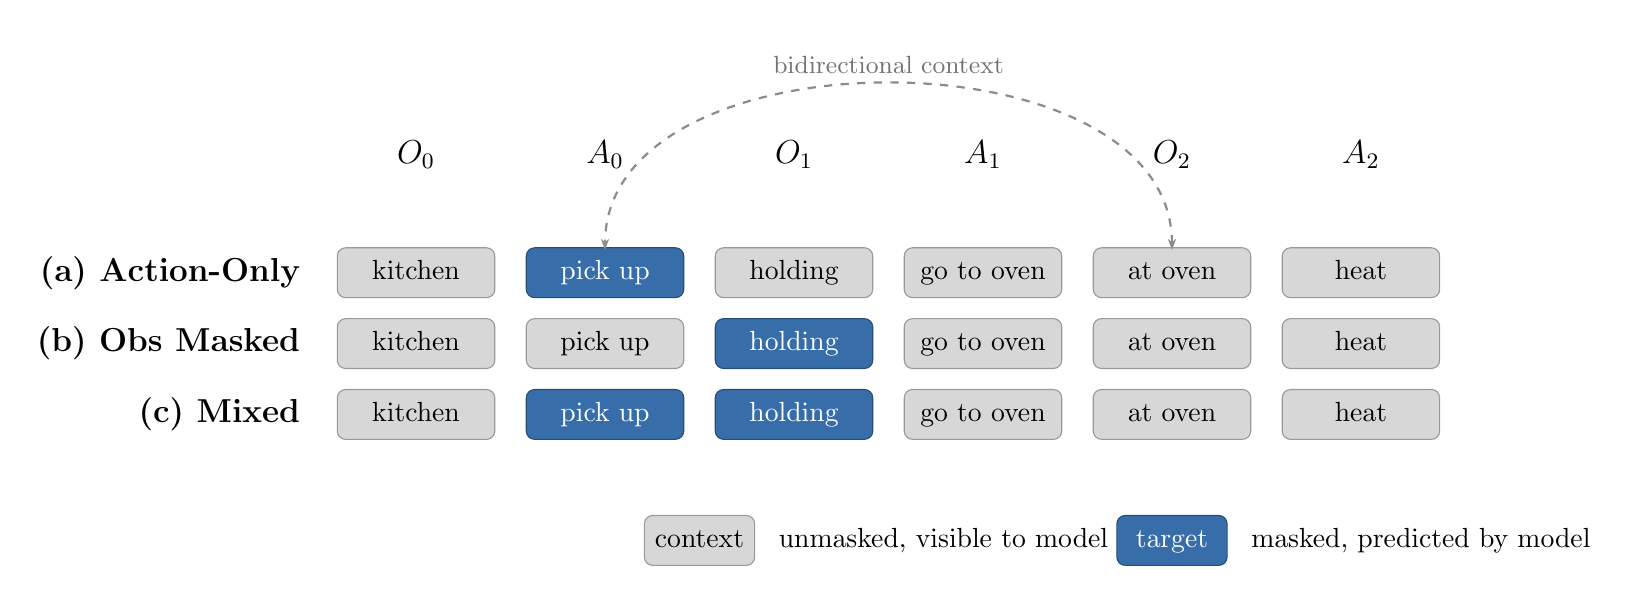
\begin{tikzpicture}[
  font=\normalsize,
  box/.style={draw, rounded corners=3pt,
              minimum width=2.0cm, minimum height=0.55cm,
              text centered, inner sep=3pt},
  ctx/.style={box, fill=ctxgray, draw=black!40},
  tgt/.style={box, fill=maskblue, draw=maskblue!70!black, text=white},
  rl/.style={font=\large\bfseries, anchor=east},
  biarr/.style={{Stealth[length=4pt]}-{Stealth[length=4pt]}, thick, dashed, black!45},
]

\def\cw{2.4}  % column width
\def\rh{0.9}  % row height

%% --- Column headers ---
\foreach \i/\lbl in {0/$O_0$, 1/$A_0$, 2/$O_1$, 3/$A_1$, 4/$O_2$, 5/$A_2$}{
  \node[font=\large\bfseries] at (\i*\cw + \cw/2, 0.6) {\lbl};
}

%% --- Row (a): Action-only masking ---
\node[rl] at (-0.15, -1*\rh) {(a) Action-Only};
\node[ctx] at (0*\cw+\cw/2, -\rh) {\strut kitchen};
\node[tgt] at (1*\cw+\cw/2, -\rh) {\strut pick up};
\node[ctx] at (2*\cw+\cw/2, -\rh) {\strut holding};
\node[ctx] at (3*\cw+\cw/2, -\rh) {\strut go to oven};
\node[ctx] at (4*\cw+\cw/2, -\rh) {\strut at oven};
\node[ctx] at (5*\cw+\cw/2, -\rh) {\strut heat};
% bidirectional context: future obs visible when predicting A0
\draw[biarr]
  (4*\cw+\cw/2, {-\rh+0.29}) to[out=90,in=90]
  node[above,midway,font=\small,black!55]{bidirectional context}
  (1*\cw+\cw/2, {-\rh+0.29});

%% --- Row (b): Observation masking ---
\node[rl] at (-0.15, -2*\rh) {(b) Obs Masked};
\node[ctx] at (0*\cw+\cw/2,-2*\rh) {\strut kitchen};
\node[ctx] at (1*\cw+\cw/2,-2*\rh) {\strut pick up};
\node[tgt] at (2*\cw+\cw/2,-2*\rh) {\strut holding};
\node[ctx] at (3*\cw+\cw/2,-2*\rh) {\strut go to oven};
\node[ctx] at (4*\cw+\cw/2,-2*\rh) {\strut at oven};
\node[ctx] at (5*\cw+\cw/2,-2*\rh) {\strut heat};

%% --- Row (c): Mixed masking ---
\node[rl] at (-0.15, -3*\rh) {(c) Mixed};
\node[ctx] at (0*\cw+\cw/2,-3*\rh) {\strut kitchen};
\node[tgt] at (1*\cw+\cw/2,-3*\rh) {\strut pick up};
\node[tgt] at (2*\cw+\cw/2,-3*\rh) {\strut holding};
\node[ctx] at (3*\cw+\cw/2,-3*\rh) {\strut go to oven};
\node[ctx] at (4*\cw+\cw/2,-3*\rh) {\strut at oven};
\node[ctx] at (5*\cw+\cw/2,-3*\rh) {\strut heat};

%% --- Legend ---
\node[ctx, minimum width=1.4cm] (lc) at (2.0*\cw, -4.3) {\strut context};
\node[right=5pt of lc, font=\normalsize] {unmasked, visible to model};
\node[tgt, minimum width=1.4cm] (lt) at (4.5*\cw, -4.3) {\strut target};
\node[right=5pt of lt, font=\normalsize] {masked, predicted by model};

\end{tikzpicture}%
}

  \caption{%
    \textbf{Unit-level mask configurations in \aomt{}} on the same ALFWorld
    trajectory.
    Blue = masked targets; white = bidirectional context.
    \emph{(a)} Action-only masking.
    \emph{(b)} Observation masking.
    \emph{(c)} Mixed masking.
    At inference, the model generates only the next action.
  }
  \label{fig:mask_illustration}
\end{figure}

\subsection{Algorithm}

\begin{algorithm}[h]
  \caption{Any-Order Masked Training (\aomt{})}
  \label{alg:aomt}
  \begin{algorithmic}[1]
    \REQUIRE Expert dataset $\Dcal$, masked DLM $p_\theta$,
             mask probability $p$, learning rate $\eta$, epochs $E$
    \FOR{epoch $= 1, \ldots, E$}
      \FOR{trajectory $\tau \in \Dcal$}
        \STATE Parse $\tau$ into unit sequence $\Ucal(\tau) = (O_0, A_0, \ldots, O_T)$
        \STATE Sample $m \sim \mathrm{Mask}(p)$ \hfill\textit{// resampled each step}
        \STATE Replace all tokens in $\Tcal(m)$ with \texttt{[MASK]}
        \STATE Forward pass with full bidirectional attention over $\Ccal(m)$
        \STATE Update $\theta \leftarrow \theta - \eta\nabla_\theta\Lcal_{\text{AOMT}}$
      \ENDFOR
    \ENDFOR
    \RETURN $\theta$
  \end{algorithmic}
\end{algorithm}

\section{Experiments}
\label{sec:experiments}

\paragraph{Benchmarks.}
We evaluate on the three-benchmark suite standard for LLM agent SFT
\citep{song2024eto,zhang2024ipr,zhang2025alee}.
\textbf{ALFWorld} \citep{shridhar2021alfworld} is a text-based household
environment (six task categories; binary success).
\textbf{ScienceWorld} \citep{wang2022scienceworld} is a science simulator with
30 task types requiring causal reasoning over 10--120 steps
(average normalised score $\times100$); the unseen split is the primary
generalisation target.
\textbf{WebShop} \citep{yao2022webshop} requires sequential product search over
12,087 items (average reward $\times100$).

\paragraph{Data.}
All experiments use the \texttt{agent-eto/eto-sft-trajectory} dataset
\citep{song2024eto}: expert ReAct trajectories with GPT-4 rationales.
No environment interaction or reward labelling is performed for any variant;
all methods train on identical data.

\paragraph{Baselines.}
\textbf{Zero-shot LLaDA~2.0-mini}: untuned base model.
\textbf{Standard SFT}: a sample-efficient baseline that mimics autoregressive
next-action prediction. Each trajectory is sliced into multiple examples,
where each action $A_t$ is masked and predicted from its full causal history
$\{O_0, A_0, \ldots, O_t\}$.
\textbf{Prefix SFT (offline IWM)}: ALEE's IWM objective adapted to an offline,
two-stage prefix-conditioning task.
Stage~1 (IWM) predicts $O_{t+1}$ from the history and $(O_t, A_t)$.
Stage~2 (Policy SFT) is then fine-tuned to predict $A_t$ from the history and $O_t$.
\textbf{\aomt{}-Action-Only}: mask restricted to action units, with the full
trajectory as bidirectional context.
\textbf{\aomt{}-Mixed} (full method): each action and observation unit
(excluding the initial objective) is masked independently with probability $p$.
ETO \citep{song2024eto}, IPR \citep{zhang2024ipr}, and Early Experience IWM
\citep{zhang2025alee} are cross-paradigm references requiring rollouts
(and rewards for ETO/IPR).

\paragraph{Model and training.}
All experiments use LLaDA~2.0-mini \citep{bie2025llada20}: 16B total / 1.4B
active parameters (MoE). Trajectories are tokenised as flat sequences with
separator tokens; unit spans are recorded at preprocessing so the mask sampler
enforces whole-unit masking. Hyperparameters: lr $2.5\times10^{-5}$ (cosine
decay to $2.5\times10^{-6}$), 50 warmup steps, weight decay 0.1, gradient
clip~1.0, batch size~64, sequence length~2048, bf16. For a fair comparison, all
experiments are trained for the same total number of gradient updates,
normalised against 3 epochs over the original unprocessed dataset.
Mask probability $p$ is swept
over $\{0.15, 0.25, 0.40, 0.50\}$ on ALFWorld and transferred to other
benchmarks. Inference: iterative unmasking, temperature~0.0, block length~32,
32 decoding steps \citep{bie2025llada20}.

\paragraph{Evaluation metrics.}
Primary metrics are task success~(\%) for ALFWorld, average normalised score for
ScienceWorld, and average reward for WebShop. We additionally report
\emph{observation-masked NLL}:
\begin{equation}
  \NLL_{\text{obs}}(\theta) =
    -\mathbb{E}_{\tau \sim \Dcal_{\text{test}}}\;
    \mathbb{E}_{t}\!\left[\log p_\theta(O_t \mid \tau \setminus O_t)\right],
  \label{eq:nll_obs}
\end{equation}
where $\tau \setminus O_t$ provides all other units as clean bidirectional
context. $\NLL_{\text{obs}}$ is a pseudo-log-likelihood
\citep{salazar2020masked} comparable across masked DLMs but incommensurable
with autoregressive log-likelihoods (Appendix~\ref{app:nll_details}).
Standard SFT and Prefix SFT are excluded from this metric.
Robustness is evaluated by randomly corrupting fraction
$\rho \in \{0.1, 0.2, 0.3\}$ of observation tokens at test time
(ALFWorld seen).

\section{Results}
\label{sec:results}

\subsection{Main Results}

Table~\ref{tab:main} compares all methods across three benchmarks.
\PLACEHOLDER{Results narrative: \aomt{}-Mixed outperforms Standard SFT on all
benchmarks; \aomt{}-Action-Only $>$ SFT isolates the bidirectional-context
benefit; \aomt{}-Mixed $>$ Action-Only on ScienceWorld unseen supports the
world-model hypothesis; gap to cross-paradigm references reflects resource
asymmetry only.}

\begin{table*}[t]
\centering
\caption{%
  \textbf{Main results.}
  Success rate (\%) for ALFWorld, average normalised score ($\times100$) for
  ScienceWorld, average reward ($\times100$) and success rate (\%) for WebShop.
  S\,/\,U = seen\,/\,unseen. All offline methods use identical training data
  and base model (LLaDA~2.0-mini).
  $\dagger$: requires environment rollouts.
  $\ddagger$: additionally requires reward signal.
  \textbf{Bold}: best offline result.
}
\label{tab:main}
\setlength{\tabcolsep}{5pt}
\begin{tabular}{lcccccc}
\toprule
& \multicolumn{2}{c}{\textbf{ALFWorld}} & \multicolumn{2}{c}{\textbf{ScienceWorld}} & \multicolumn{2}{c}{\textbf{WebShop}} \\
\cmidrule(lr){2-3}\cmidrule(lr){4-5}\cmidrule(lr){6-7}
\textbf{Method} & S & U & S & U & Rew. & Succ. \\
\midrule
\multicolumn{7}{l}{\textit{Cross-paradigm references (additional resources required)}} \\[1pt]
Early Exp.\ IWM$^\dagger$ \citep{zhang2025alee}  & \PLACEHOLDER{XX.X} & \PLACEHOLDER{XX.X} & \PLACEHOLDER{XX.X} & \PLACEHOLDER{XX.X} & \PLACEHOLDER{XX.X} & \PLACEHOLDER{XX.X} \\
ETO$^{\dagger\ddagger}$ \citep{song2024eto}       & \PLACEHOLDER{XX.X} & \PLACEHOLDER{XX.X} & \PLACEHOLDER{XX.X} & \PLACEHOLDER{XX.X} & \PLACEHOLDER{XX.X} & --- \\
IPR$^{\dagger\ddagger}$ \citep{zhang2024ipr}      & \PLACEHOLDER{XX.X} & \PLACEHOLDER{XX.X} & \PLACEHOLDER{XX.X} & \PLACEHOLDER{XX.X} & \PLACEHOLDER{XX.X} & --- \\
\midrule
\multicolumn{7}{l}{\textit{Offline SFT methods (no rollouts, no reward)}} \\[1pt]
Zero-shot LLaDA~2.0-mini                          & \PLACEHOLDER{XX.X} & \PLACEHOLDER{XX.X} & \PLACEHOLDER{XX.X} & \PLACEHOLDER{XX.X} & \PLACEHOLDER{XX.X} & \PLACEHOLDER{XX.X} \\
Standard SFT                                       & \PLACEHOLDER{XX.X} & \PLACEHOLDER{XX.X} & \PLACEHOLDER{XX.X} & \PLACEHOLDER{XX.X} & \PLACEHOLDER{XX.X} & \PLACEHOLDER{XX.X} \\
Prefix SFT (offline IWM)                           & \PLACEHOLDER{XX.X} & \PLACEHOLDER{XX.X} & \PLACEHOLDER{XX.X} & \PLACEHOLDER{XX.X} & \PLACEHOLDER{XX.X} & \PLACEHOLDER{XX.X} \\
\aomt{}-Action-Only                                & \PLACEHOLDER{XX.X} & \PLACEHOLDER{XX.X} & \PLACEHOLDER{XX.X} & \PLACEHOLDER{XX.X} & \PLACEHOLDER{XX.X} & \PLACEHOLDER{XX.X} \\
\aomt{}-Mixed \textbf{(ours)}                      & \PLACEHOLDER{\textbf{XX.X}} & \PLACEHOLDER{\textbf{XX.X}} & \PLACEHOLDER{\textbf{XX.X}} & \PLACEHOLDER{\textbf{XX.X}} & \PLACEHOLDER{\textbf{XX.X}} & \PLACEHOLDER{\textbf{XX.X}} \\
\bottomrule
\end{tabular}
\end{table*}

\subsection{Ablations}

Table~\ref{tab:ablation_p} sweeps mask probability $p$ on ALFWorld.
Table~\ref{tab:ablation_type} isolates the contributions of bidirectional context
and world-model training independently.
\PLACEHOLDER{Ablation narrative: intermediate $p \in [0.25, 0.40]$ expected
optimal; world-model benefit largest on ScienceWorld unseen.}

\begin{table}[h]
\centering
\caption{\textbf{Mask probability ablation} on ALFWorld (success rate \%).}
\label{tab:ablation_p}
\begin{tabular}{lcc}
\toprule
$p$ & Seen & Unseen \\
\midrule
0.15 & \PLACEHOLDER{XX.X} & \PLACEHOLDER{XX.X} \\
0.25 & \PLACEHOLDER{XX.X} & \PLACEHOLDER{XX.X} \\
0.40 & \PLACEHOLDER{XX.X} & \PLACEHOLDER{XX.X} \\
0.50 & \PLACEHOLDER{XX.X} & \PLACEHOLDER{XX.X} \\
\midrule
Standard SFT (ref.) & \PLACEHOLDER{XX.X} & \PLACEHOLDER{XX.X} \\
\bottomrule
\end{tabular}
\end{table}

\begin{table}[h]
\centering
\caption{%
  \textbf{Masking type ablation.}
  ALFWorld success rate (\%) and ScienceWorld unseen ($\times100$).
}
\label{tab:ablation_type}
\begin{tabular}{lccc}
\toprule
& \multicolumn{2}{c}{ALFWorld} & SciWorld \\
\cmidrule(lr){2-3}\cmidrule(lr){4-4}
\textbf{Method} & Seen & Unseen & Unseen \\
\midrule
Standard SFT        & \PLACEHOLDER{XX.X} & \PLACEHOLDER{XX.X} & \PLACEHOLDER{XX.X} \\
\aomt{}-Action-Only & \PLACEHOLDER{XX.X} & \PLACEHOLDER{XX.X} & \PLACEHOLDER{XX.X} \\
\aomt{}-Mixed       & \PLACEHOLDER{XX.X} & \PLACEHOLDER{XX.X} & \PLACEHOLDER{XX.X} \\
\bottomrule
\end{tabular}
\end{table}

\subsection{World-Model Quality and Robustness}

Table~\ref{tab:nll} reports $\NLL_{\mathrm{obs}}$ for the two \aomt{} variants;
Table~\ref{tab:robustness} evaluates task success under observation-token
corruption.
\PLACEHOLDER{\aomt{}-Mixed achieves lower $\NLL_{\mathrm{obs}}$ and degrades
more gracefully under noise, consistent with joint world-model training.}

\begin{table}[h]
\centering
\caption{%
  \textbf{Observation-masked NLL} ($\downarrow$ better).
  Pseudo-log-likelihood \citep{salazar2020masked}; comparable across masked
  DLMs only. SFT variants excluded (see Appendix~\ref{app:nll_details}).
}
\label{tab:nll}
\begin{tabular}{lccc}
\toprule
\textbf{Method} & ALFWorld & SciWorld & WebShop \\
\midrule
Standard SFT        & ---                         & ---                         & ---                         \\
Prefix SFT          & ---                         & ---                         & ---                         \\
\aomt{}-Action-Only & \PLACEHOLDER{X.XX}          & \PLACEHOLDER{X.XX}          & \PLACEHOLDER{X.XX}          \\
\aomt{}-Mixed       & \PLACEHOLDER{\textbf{X.XX}} & \PLACEHOLDER{\textbf{X.XX}} & \PLACEHOLDER{\textbf{X.XX}} \\
\bottomrule
\end{tabular}
\end{table}

\begin{table}[h]
\centering
\caption{%
  \textbf{Robustness under observation noise.}
  ALFWorld (seen) success rate (\%) with fraction $\rho$ of observation tokens
  randomly corrupted at test time.
}
\label{tab:robustness}
\begin{tabular}{lccc}
\toprule
\textbf{Method} & $\rho{=}0.1$ & $\rho{=}0.2$ & $\rho{=}0.3$ \\
\midrule
Standard SFT        & \PLACEHOLDER{XX.X} & \PLACEHOLDER{XX.X} & \PLACEHOLDER{XX.X} \\
\aomt{}-Action-Only & \PLACEHOLDER{XX.X} & \PLACEHOLDER{XX.X} & \PLACEHOLDER{XX.X} \\
\aomt{}-Mixed       & \PLACEHOLDER{XX.X} & \PLACEHOLDER{XX.X} & \PLACEHOLDER{XX.X} \\
\bottomrule
\end{tabular}
\end{table}

\subsection{Analysis}

\paragraph{World-model quality vs.\ task success.}
Figure~\ref{fig:nll_vs_success} plots $\NLL_{\mathrm{obs}}$ against ScienceWorld
unseen task success across checkpoints (every 500 steps) for both \aomt{}
variants. The two-variant design tests whether better $\NLL_{\mathrm{obs}}$
predicts generalisation at matched task success levels, avoiding conflation with
training progress.

\begin{figure}[h]
  \centering
  \figplaceholder[4cm]{Scatter: NLL$_\text{obs}$ vs.\ ScienceWorld unseen task
    success. One point per checkpoint (500-step intervals), both \aomt{} variants.
    Pearson $r$ and $p$-value annotated. Generated after experiments.}
  \caption{%
    \textbf{$\NLL_{\mathrm{obs}}$ vs.\ ScienceWorld unseen task success.}
    \PLACEHOLDER{Fill in correlation statistics.}
    Points from both \aomt{} variants; one per checkpoint.
  }
  \label{fig:nll_vs_success}
\end{figure}

\paragraph{Attention patterns.}
To verify that \aomt{}-Mixed exploits bidirectional context, we extract
final-layer attention weights averaged over 50 held-out trajectories when
reconstructing a masked mid-trajectory action. Standard SFT (causal mask) serves
as a zero-future-attention reference. Full heatmaps are in Appendix~\ref{app:attention}.
\PLACEHOLDER{Describe key finding: AOMT-Mixed attends substantially to future
units; Standard SFT does not.}

\paragraph{Failure mode analysis.}
\PLACEHOLDER{Brief summary of 3--5 cases where \aomt{}-Mixed succeeds and
Standard SFT fails on ScienceWorld unseen, with the key piece of bidirectional
context that distinguishes them. Full table in Appendix~\ref{app:failures}.}

\section{Conclusion}
\label{sec:conclusion}

We introduced Any-Order Masked Training (\aomt{}), a reward-free offline SFT
paradigm for LLM-based agents that treats training-order assignment as a
variable rather than a fixed commitment. By resampling unit-level masks across
epochs and reconstructing masked trajectory spans from bidirectional context,
\aomt{} extracts a richer family of supervisory signals from a fixed expert
corpus than any single-order method. We proved that standard SFT and offline
ALEE-IWM are degenerate special cases under constrained mask samplers, and
introduced observation-masked NLL as a natural evaluation metric for implicit
world-model quality.
\PLACEHOLDER{Summarise key empirical findings: (1) \aomt{}-Mixed outperforms SFT
across all benchmarks; (2) bidirectional context and world-model training
contribute independently; (3) $\NLL_{\mathrm{obs}}$ correlates with task success
on ScienceWorld but not WebShop; (4) \aomt{}-Mixed degrades more gracefully under
observation noise.}

\paragraph{Limitations and future work.}
\aomt{} currently operates on text-based trajectories; extension to visual
observations requires unit-level masking over image patches, building on
multimodal masked DLMs \citep{zhou2025lladav}. The formal relationship between
\aomt{}'s unit-level objective and LLaDA's ELBO warrants further analysis
(Appendix~\ref{app:elbo}). The most immediate extension is composing \aomt{}
with ALEE's data-collection pipeline---applying any-order masked reconstruction
to agent-generated rollouts to address both data-diversity and objective-richness
bottlenecks simultaneously.

\paragraph{Broader impact.}
\aomt{} improves sample efficiency of SFT on fixed offline corpora without
requiring additional environment interaction or reward labelling. Risks are those
generic to improved LLM-agent capabilities.


\bibliography{references}

\newpage
\appendix
\section*{Appendix}
\setcounter{section}{0}
\renewcommand{\thesection}{\Alph{section}}

\section{Proofs}
\label{app:proofs}

\begin{proof}[Proof of Proposition~\ref{prop:subsumption}]
\textbf{(i) Standard SFT.}
Fix $m$ to always mask exactly one action unit $A_t$, with context
$\Ccal(m) = \{O_0, A_0, \ldots, O_t\}$ and a causal attention mask preventing
any future unit from contributing to the reconstruction of $A_t$.
Substituting into Eq.~\eqref{eq:aomt}:
\[
  \Lcal_{\text{AOMT}}(\tau,m) = -\log p_\theta(A_t \mid O_0, A_0, \ldots, O_t),
\]
which is exactly the standard SFT loss summed over $t = 0,\ldots,T-1$.

\textbf{(ii) Offline ALEE-IWM.}
Fix $m$ to always mask $O_{t+1}$, with context $\Ccal(m) = \{O_t, A_t\}$
(local context only).
Substituting into Eq.~\eqref{eq:aomt}:
\[
  \Lcal_{\text{AOMT}}(\tau,m) = -\log p_\theta(O_{t+1} \mid O_t, A_t),
\]
which is the ALEE-IWM loss restricted to the offline expert corpus.
\aomt{} with an unconstrained Bernoulli($p$) sampler strictly generalises both
by allowing any subset of units to be masked and using full bidirectional
attention over all context units.
\end{proof}

\section{Relationship to Masked Diffusion ELBO}
\label{app:elbo}

LLaDA \citep{nie2025llada} trains with:
\begin{equation}
  \Lcal_{\text{LLaDA}} = -\mathbb{E}_{t \sim U[0,1]}\,
    \mathbb{E}_{m \sim \mathrm{Mask}(t)}\,
    \frac{1}{t} \sum_{i : m_i=1} \log p_\theta(x_i \mid x \odot (1-m)),
\end{equation}
a variational upper bound on token-level NLL.
\aomt{} replaces token-level masking with unit-level masking and fixes the
schedule to a single probability $p$, trading the ELBO interpretation for a
cleaner semantic objective aligned with agent decision granularity.
We conjecture that \aomt{} inherits Fisher consistency from LLaDA at the unit
level; formal proof is left to future work.

At inference, \aomt{} uses LLaDA~2.0's block diffusion decoding (iterative
unmasking over 32 steps), not single-pass reconstruction. The any-order
learning effect emerges from mask diversity \emph{across training steps},
not within-trajectory iterative refinement.

\section{Observation-Masked NLL: Implementation Details}
\label{app:nll_details}

As LLaDA predicts each masked token independently in a single forward pass,
$\NLL_{\text{obs}}$ (Eq.~\eqref{eq:nll_obs}) is a \emph{pseudo-log-likelihood}
in the sense of \citet{salazar2020masked}: it sums per-token log-probabilities
assuming conditional independence of tokens in $O_t$ given context, rather than
computing the true joint $\log p(O_t \mid \tau \setminus O_t)$. It is directly
comparable across masked DLM checkpoints but not commensurable with
autoregressive log-likelihoods, which condition only on past context and
therefore measure forward prediction rather than bidirectional world-model quality.

Standard SFT and Prefix SFT Stage~1 are excluded from $\NLL_{\text{obs}}$
tables: the former has no mechanism for future conditioning; the latter was
trained with single-step context $(O_t, A_t)$ only, making full-trajectory
evaluation out-of-distribution.

\section{Attention Heatmaps}
\label{app:attention}

\PLACEHOLDER{Final-layer attention weights averaged across all heads over 50
held-out ALFWorld trajectories, when reconstructing a masked mid-trajectory
action. Left: \aomt{}-Mixed. Right: Standard SFT (zero-future-attention
reference). AOMT-Mixed is expected to show substantial weight on future context
units; Standard SFT should show none. Generated after experiments complete.}

\section{Failure Mode Analysis}
\label{app:failures}

\PLACEHOLDER{Table of 3--5 representative cases where \aomt{}-Mixed succeeds
and Standard SFT fails on ScienceWorld unseen tasks. For each case: task
description, step at which SFT diverges, SFT's incorrect action,
\aomt{}-Mixed's correct action, and the key piece of bidirectional context
that distinguishes them.}

\section{Full Results by Task Category}
\label{app:full_results}

\PLACEHOLDER{Per-category breakdown of ALFWorld results (all six task types)
and ScienceWorld results (all 30 task types) for all offline methods.}


\end{document}
